\documentclass[10pt,a4paper]{article}
\usepackage[T1]{fontenc}
\usepackage[scaled]{helvet}
\usepackage{cite}
\usepackage{url}
\usepackage{graphicx}
\usepackage{listings}
\usepackage{float}
\usepackage{amsmath}
\usepackage{listings}
\usepackage{color}
 
\definecolor{dkgreen}{rgb}{0,0.6,0}
\definecolor{gray}{rgb}{0.5,0.5,0.5}
\definecolor{mauve}{rgb}{0.58,0,0.82}
\lstset{ %
  language=Octave,                % the language of the code
  basicstyle=\footnotesize,           % the size of the fonts that are used for the code
  numbers=left,                   % where to put the line-numbers
  numberstyle=\tiny\color{gray},  % the style that is used for the line-numbers
  stepnumber=1,                   % the step between two line-numbers. If it's 1, each line 
                                  % will be numbered
  numbersep=5pt,                  % how far the line-numbers are from the code
  backgroundcolor=\color{white},      % choose the background color. You must add \usepackage{color}
  showspaces=false,               % show spaces adding particular underscores
  showstringspaces=true,         % underline spaces within strings
  showtabs=false,                 % show tabs within strings adding particular underscores
  frame=none,                   % adds a frame around the code
  rulecolor=\color{black},        % if not set, the frame-color may be changed on line-breaks within not-black text (e.g. commens (green here))
  tabsize=2,                      % sets default tabsize to 2 spaces
  breaklines=true,                % sets automatic line breaking
  breakatwhitespace=false,        % sets if automatic breaks should only happen at whitespace
  keywordstyle=\color{blue},          % keyword style
  commentstyle=\color{dkgreen},       % comment style
  stringstyle=\color{mauve},         % string literal style
  escapeinside={\%*}{*)},            % if you want to add LaTeX within your code
  morekeywords={*,...}               % if you want to add more keywords to the set
}
\usepackage{amssymb}
\usepackage{fancyhdr}
\usepackage{lastpage}
\floatstyle{boxed} 
\restylefloat{figure}
\renewcommand*\familydefault{\sfdefault}
\title{Process Synchronization and Co-ordination}
\author{David Lynch - david.lynch@raglansoftware.com }
\begin{document}
\maketitle
\begin{abstract}
To date we have talked about concurrently running threads of execution, but have not addressed any of the fundamental protections that must be afforded to state that is shared between different threads. We have already alluded to a number of problems with data consistency and determinism that are surfaced by multi-threaded execution. This article examines these issues in detail and discusses some protections that operating systems provided to mitigate against these issues.
\end{abstract}
\section{The Critical Section}
Where several processes or threads access and manipulate the same data concurrently, and the output is dependent on the order in which the operations take place we have a {\bf race condition}. Synchronization and co-ordination is concerned with how interacting threads or processes can protect against the incorrect or inconsistent outputs this condition has the potential to produce. Synchronization mechanisms are concerned with the timing of execution of multiple actions on shared state. Co-ordination is concerned with signalling between processes that share that particular state. A {\bf critical section} is a segment of code in a process where the process changes some common resource or state. A protocol must exist whereby each process must request permission to enter the critical section. The point at which this protocol is used is known as the {\bf entry section}. The end of a critical section is demarcated by the {\bf exit section}. The code that executes after the exit section is known as the {\bf remainder section}.
\subsection{Example}
Consider a Java program that simulates facilities in a bank. By their very nature, different facilities run concurrently. From the customer perspective, I must be able to withdraw money from my account at all times including when other transactions are being applied to my account. Figures  \ref{jbankapp},\ref{jaccount},\ref{jatm},\ref{jcredit} and \ref{jfacility} show the full implementation and figure \ref{bad-results} shows the aggregated results after 100 executions.  We can clearly see there is a race condition here, as the results of this application are not consistent over multiple runs. Moreover, in unit testing, or otherwise ill-considered testing, this may be a tricky thing to spot. In fact, in general, debugging and designing multi-threaded applications is a tricky process that requires investment in time and an excellent understanding. 
\newline\newline
This race condition is caused by the scheduler. In particular, lines 17 and 21 of {\it Account.java} in figure \ref{jaccount}. These are the lines that explicitly mutate the balance of of the account. Figure \ref{byte-code} shows the byte-code that is generated by the line 10 in {\it Account.java}. Note that there are several distinct operations that are happening here, each of which is {\bf atomic}. The saving of the results of the operation back to the variable is a distinct operation from the addition of funds to the balance. Remember, threads will share a text-section. If the scheduler is switched out before the results of the operation have been written back, and the context switch results in a read of the balance, the resulting write-back may override the results of the original operation. To assist the scheduler, and prevent this operation from causing negative side-effects, we can instruct the JVM to demarcate critical sections of code, facilitating {\bf atomicity} of sets of operations on that state. An atomic operation will either execute in full, or not execute at all. In Java, the {\bf synchronized} keyword is used to obtain a {\bf lock} on the shared state at the class level. This is the minimum level of locking in Java. Figures \ref{jcredit-synch} and \ref{jatm-synch} illustrates how we can control entry to this critical section in Java. The curly braces indicate the scope of the critical section and the brackets indicate the resource around which the critical section will synchronize. The first is the entry section and the final brace the exit section. No other thread that needs a lock on this state will be allowed to enter its critical section until this lock is released. 
\newline\newline
The general terms for the problem illustrated here are encapsulated by the terms {\bf dirty read} and {\bf lost update}. A dirty read occurs when the incomplete results of concurrent operation are read by another thread. A lost update occurs when the results of a concurrent operation are overwritten by the inconsistent results of another operation. By ensuring we demarcate both critical sections using the synchronized keyword to lock around the Account object, we protect ourselves against both of these scenarios and ensure the results of our concurrent executions are correct and consistent. In essence, the Account object is a monitor against which only one thread my execute any operation. 
\newline\newline
It is extremely important that you understand everything that has been explained here in full detail before moving on. With respect to race conditions in accesses to shared state, this is  as simple as it gets. Needless to say, things do, and will, get much more complex. Spend the time understanding everything from the actual problem that is being solved, the threads under execution and how they are managed in the operating system, every line of the listings show and the Java byte code. It is a worthwhile exercise to replicate the demonstration of this problem given in class. Experiment with what happens when the synchronized block is removed from only one of the facilities. Explore other ways of achieving the same effect, for example by using synchronized methods. You can check out the source code from \cite{GITHUB}. It is recommended that you do this and play around with the example.
\begin{figure}
\caption{Java Implementation of a Bank Account}
\begin{center}
\lstinputlisting[language=Java]{../listings/bank/Account.java}
\label{jaccount}
\end{center}
\end{figure}

\begin{figure}
\caption{An abstract Bank Facility}
\begin{center}
\lstinputlisting[language=Java]{../listings/bank/BankFacility.java}
\label{jfacility}
\end{center}
\end{figure}

\begin{figure}
\caption{An ATM Facility which executes some withdrawals.}
\begin{center}
\lstinputlisting[language=Java]{../listings/bank/ATMWithdrawalFacility.java}
\label{jatm}
\end{center}
\end{figure}

\begin{figure}
\caption{A credit transfer facility executing some deposits.}
\begin{center}
\lstinputlisting[language=Java]{../listings/bank/CreditTransferFacility.java}
\label{jcredit}
\end{center}
\end{figure}

\begin{figure}
\caption{A bank application with concurrently running facilities.}
\begin{center}
\lstinputlisting[language=Java]{../listings/bank/BankExample.java}
\label{jbankapp}
\end{center}
\end{figure}

\begin{figure}
\caption{A safer implementation of listing \ref{jatm}}
\begin{center}
\lstinputlisting[language=Java]{../listings/bank/SynchATMWithdrawalFacility.java}
\label{jatm-synch}
\end{center}
\end{figure}

\begin{figure}
\caption{A safer implementation of listing \ref{jcredit}}
\begin{center}
\lstinputlisting[language=Java]{../listings/bank/SynchCreditTransferFacility.java}
\label{jcredit-synch}
\end{center}
\end{figure}



\begin{figure}
\caption{Differing final states show the effects of a race condition.}
\begin{center}
\begin{lstlisting}
	Count   Final Balance
      1 	1050.0
      1 	170.0
      2 	160.0
     96 	1140.0
\end{lstlisting}
\label{bad-results}
\end{center}
\end{figure}

\begin{figure}
\caption{Java bytecode decomplication of the deposit method in listing \ref{jaccount}}
\begin{center}
\begin{lstlisting}
public void deposit(double);
  Code:
   0:	aload_0
   1:	dup
   2:	getfield	#15; //Field balance:D
   5:	dload_1
   6:	dadd
   7:	putfield	#15; //Field balance:D
   10:	return
\end{lstlisting}
\label{byte-code}
\end{center}
\end{figure}

\subsection{The Critical Section Problem}
We now move back from the implementation, to the abstract concepts at an OS level. We can generalise synchronization in Java to a critical section problem that needs to be solved by enforcing three principles.  
\subsubsection{Mutual Exclusion}
In any process critical sections can be drawn across threads internally and across relationships with other processes along a line that is connected with access to the same shared state. When we make a particular critical section mutually exclusive, then we ensure that no other process, or thread is executing either its copy of the critical section code, or code that will access shared state in a dangerous way concurrently. 
\subsubsection{Progress}
Mutual exclusion is simple. We can associate a marker or a {\bf lock} that can be acquired {\bf atomically} with the resource that we are intending to restrict access. However, we must provide a facility to ensure that these locks are acquired and released correctly, or otherwise a process may never proceed. In order to mitigate this, we enforce the principle of progress. Only processes that are not executing their remainder sections can participate in the decision for a process to enter its critical section, and this decision cannot be deferred indefinitely. 
\subsubsection{Bounded Waiting}
This is the final principle, and it states that there is a limit on the number of times that can enter its critical sections after a process has made a request to enter its critical section and before the request to enter is granted. This ensures, in some way, fairness. In simpler terms, if I wish to acquire a lock on a resource, any facility that solves the critical section problem, will guarantee that at some point, I will be able to acquire that lock. 
\subsubsection{Petersons Solution}
Gary Peterson et al. \cite{Peterson} proposed a solution to management of critical sections that can be disseminated into the the listing in figure \ref{plisting}. The entry section guarantees mutual exclusion by ensuring that the process will not enter the critical section until it has been instructed to do so by the other process. Progress is guaranteed since when the process re-enters its critical section it immediately yields to other processes. Lastly, bounded waiting is enforced due to the fact that one execution of the section will happen at most before the critical section of another process is executed. Figure \ref{plisting} implements what is commonly referred to as a {\bf spin-lock}. While simple to implement, spin-locks are {\bf busy waits} and consume CPU while doing very little. Some more advanced approaches to locking involve explicit signalling that may wake up a thread from sleeping. Figure \ref{plisting} is also a primitive implementation of what is known as a {\bf mutex}.
\begin{figure}
\caption{Pseudo-code that illustrates the approach taken by Peterson in \cite{Peterson}}
\begin{center}
\begin{lstlisting}
do {
	/// ENTRY SECTION ///

	/** Express interest on the critical section */
	flag[thisThread] = true;
	
	/** Yield immediately */
	turn 			 = otherTread;
	
	/** Spin until the lock is acquired */
	while (flag[otherThread] && turn == otherThread) {
		/* SPIN */
	}
	
	/// CRITICAL SECTION ///
	/** Execute Critical Section */
	
	/// EXIT SECTION ///
	/** Release the lock */
	flag[thisThread] = false;
	
	/// REMAINDER SECTION ///
} while (true);
\end{lstlisting}
\label{plisting}
\end{center}
\end{figure}
\subsection{Semaphores}
Petersons approach as illustrated in listing \ref{plisting} can become somewhat onerous to implement, particularly when multiple threads can acquire the same lock. A  {\bf semaphore} is a means by which access to a shared resource can be restricted, but not necessarily mutually exclusively. Also, it provides a better level of abstraction when coding around critical sections. The atomic operations {\bf wait} and {\bf signal} provide the interface to the semaphore. A count is maintained and is limited at the maximum number of entities that can hold the resource. If the maximum value of this count is 1 this primitive reduces to a mutex. Figure illustrates a simple implementation of the semaphore. For two concurrently running processes with operation $S_1$ for $P_1$ and operation $S_2$ for $P_2$, we can ensure that $S_2$ is only executed after $S_1$ by making $S_2$ wait on a lock from $S_1$ and ensuring that $S_1$ signals upon completion of its critical section. Figure \ref{lsemaphore} illustrates the above concepts in pseudo-code.
\begin{figure}
\caption{Pseudo-Code for implementation and use of a semaphore \cite{OSCONCEPTS}}
\begin{center}
\begin{lstlisting}
wait (S) {
	while S <= 0 { // no-op };
	S--;
}

signal(S) {
	S++;
}

do {
	wait(S);
	// CRITICAL SECTION
	signal(S);
} while (true);
\end{lstlisting}
\label{lsemaphore}
\end{center}
\end{figure}
\subsection{Monitors}
A monitor is an abstract data-type, or class, that presents public access to private data in a controlled manner. It is functionally similar to a mutex, allowing only one thread of execution enter a critical section associated with some resource at a time. Typically a queue of interested threads is maintained and only one thread allowed to invoke operations on that monitor at any one time. In Java, each object is a monitor. Control of invocation of methods on an object can be obtained exclusively using the synchronized keyword, as shown earlier in this article. In fact, we solved our race condition problem through use of a monitor in Java as we instructed each thread to acquire exclusive access to all of each objects methods while we were in the critical section of code that mutated the account balance. For more on Monitors in Java see \cite{JAVASYNC}. 
\section{Deadlock and Inter-Thread Co-ordination}
With multiple threads waiting in a queue on multiple resources, we can end up in a situation where two or more processes are waiting indefinitely for an event that can only be caused by one of the waiting processes in the queue. This situation is known as {\bf deadlock}. Figure \ref{deadlock} shows a schedule with two processes, each waiting on another to release a lock owned by the other. A very similar concept is {\bf livelock}, whereby the states of all of the members of the queue are constantly changing with respect one another. They are not waiting, but in the main, no progression is made. This is a special case of {\bf starvation}, whereby a process progression is hampered due to its inability to get a lock on the resource that it needs to progress, typically due to the resource being held by other processes at various times during its wait period. This typically happens if the queueing strategy is last-in-first out, and the queue never gets time to empty. 
\begin{figure}
\caption{A deadlocked schedule with two processes}
\begin{center}
\begin{tabular}{| l | l | }
  \hline
  P0 & P1 \\ \hline
  wait(S) & wait(Q) \\
  wait(Q) & wait(S) \\
  .. & .. \\
  signal(S) & signal(Q) \\
  signal(Q)	& signal(S) \\
  \hline
\end{tabular}
\label{deadlock}
\end{center}
\end{figure}
\subsection{The Dining Philosophers Problem}
This is a well documented analogy that demonstrates the need to allocate resources in a deadlock free manner across competing resources. Philosophers  can be in one of two states, thinking or eating. They all sit at a round table and are sharing a bowl of rice. They cannot communicate with each other by thinking. When hungry, they may only acquire one chopstick at a time. When no longer hungry, each philosopher puts down both of his chopsticks. There are five chopsticks at a table of five philosophers, all sharing one bowl of rice. Each philosopher needs two chopsticks to eat. If there were no strategy to ensure progress, a deadlock situation could occur in a number of ways. If all philosophers become hungry at the same time, and each pick up the right chopstick first, there will be an indefinite wait on the right chopstick. This is a deadlock. If three philosophers are particularly hungry, they may acquire the chopsticks, leaving the other philosophers starving. If we restrict holding a single chopstick to a period of time, such that if we do not require a second chopstick in that time we release the single chopstick, then we are open to an interleaved wait-release cycle. This is a live-lock. 
\subsubsection{Semaphore Solution}
Introduce a waiter to the table. Each philosopher must ask the permission of the waiter before any chopsticks are lifted up. Since the waiter will track the amount of chopsticks available and in use, he acts as an arbitrator in preventing deadlock. Practically, the waiter is implemented as a semaphore across the 5 chopsticks. The additional constraint that unless a philosopher can acquire two forks atomically, then the philosopher must release any existing fork is added to the rule-set. Further modifications can be made to this algorithm to decrease the likelihood of starvation, such as limiting the amount of time for which a chopstick can be  held. 
\subsubsection{Other Solutions}
There is at least one other solution that can be implemented when the ability for philosophers to talk to each other is added. You should look this up and understand it before continuing.
\begin{figure}
\caption{Dining Philosophers at a Table \cite{OSCONCEPTS}}
\begin{center}
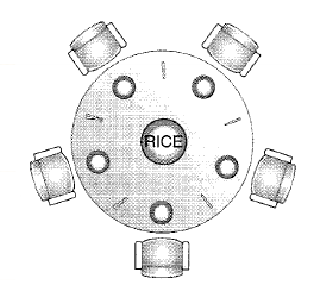
\includegraphics[scale=0.45]{../images/dining.png}
\label{os}
\end{center}
\end{figure}
\subsection{The Bounded Buffer Problem}
This is also known as the producer consumer problem. There is a producer of work, a consumer of work and a shared queue. The producer and consumer both run concurrently. The consumer removes data from the queue, while the producer adds new work to the queue. We need to ensure that the producer does not try to add data to a full buffer. Similarly, the producer should not remove data from an empty queue. Lastly, we need to ensure that both processes do not deadlock or starve. The only way to correctly manage this problem is to supplement standard synchronization primitives such as locks with the ability of threads to communicate with one another. In the case of Java, we use the {\bf wait} and {\bf notify} invocations on the shared Queue's monitor. The thread safe queue in listing \ref{jqueue} shows how both enqueue and dequeue can be correctly implemented so that there is no deadlock. If the queue is not full the producer \ref{jproducer} will keep pushing data onto the queue. Concurrently, the consumer \ref{jconsumer} will be switched in periodically to empty the queue. When the queue is full, the consumer will not attempt to push any more data onto the queue but instead blocks on acquiring the monitor on the Queue. This causes the producer to wait until some invocation of notify on the Queue monitor. Since the consumer invokes notify after a successful dequeue, the producer will then wake up and acquire the monitor that the consumer has release. Note that the only time the monitor is acquired is when a wait is required. In the cases of normal production to a non-full queue and normal emptying of a non-full queue, neither the producer and consumer are concerned with co-ordination. However, at this time, synchronization is still important, in particular around the pointer that demarcates the head and the tail of the buffer. The synchronized nature of the method provides protection against lost updates and dirty reads as outlined before. 
\newline\newline
The producer consumer problem illustrates important concepts in synchronization and, in particular, co-ordination between threads. Please do not move on until you fully understand the Java code and how the Monitor works. You can check out the code from \cite{GITHUB} and play with it. Try removing synchronized keywords, or removing the waits. Try reworking the problem to work with multiple producers and consumers. 

\begin{figure}
\caption{Java implementation of a consumer}
\begin{center}
\lstinputlisting[language=Java]{../listings/prodconsumer/Consumer.java}
\label{jconsumer}
\end{center}
\end{figure}

\begin{figure}
\caption{Java implementation of a consumer}
\begin{center}
\lstinputlisting[language=Java]{../listings/prodconsumer/Producer.java}
\label{jproducer}
\end{center}
\end{figure}

\begin{figure}
\caption{A thread-safe bounded buffer in Java.}
\begin{center}
\lstinputlisting[language=Java]{../listings/prodconsumer/Queue.java}
\label{jqueue}
\end{center}
\end{figure}

\begin{figure}
\caption{A simple Unit of Work}
\begin{center}
\lstinputlisting[language=Java]{../listings/prodconsumer/UnitOfWork.java}
\label{junit}
\end{center}
\end{figure}

\begin{figure}
\caption{Producer consumer problem main program.}
\begin{center}
\lstinputlisting[language=Java]{../listings/prodconsumer/ProducerConsumerProblem.java}
\label{jprodconsumer}
\end{center}
\end{figure}

\section{Transactions and Atomicity}
A transaction is a single unit of work that is either performed in its entirety or not performed at all. If a transaction is completed in its entirety it is said to be {\bf committed}. If the transaction is not completed it is said to be aborted. To ensure atomicity, the effects of aborted transactions must be {\bf rolled back}. This ensures consistency by leaving the system in the same state as it appeared before it entered the transaction.  
\subsection{Log Based Recovery}
In order to support rollback  of changes to volatile memory is to log all modifications. Write-ahead logging uses log entries to record data about the modification. This will include a unique transaction id, the old value and the new value. Everything in this case is recorded to stable storage before volatile storage is modified. There is a performance penalty, the cost being more complexity and more storage costs. The advantage is the ability to undo the transaction by reversing the log, and transactions can be replayed  by playing the log forward. 
\subsection{Checkpoints}
The disadvantage of explicit logging is that replaying the log may be redundant for some or a lot of transactions. Determining which transactions need to be redone and which need to be rolled back is a search problem and can be costly. Checkpointing will set explicit safe points at which all records in volatile memory are outputted to stable storage. When just after a checkpoint is logged, everything is fully consistent. To get to the last stable consistent state, only the last checkpoint need to be reloaded. However, due to the fact we do no log at the point of every operation, data can still be lost between checkpoints. 
\subsection{Concurrent Atomic Transactions}
The effects of transactions that execute concurrently must be exactly the same as the effects if these transactions were execute serially. With multiple concurrently executing transactions, particularly on areas of data that are highly shared, exposing a single mutex is not often the best strategy. Essentially, the mutex becomes the focal point of the transaction and the amount of time any concurrently executing transaction waits around on the mutex not optimal. There are properties of transactions that can be leveraged to achieve consistency in the presence of concurrency without reducing concurrency to serial execution. 
\newline\newline
Concurrent transactions are executed in a {\bf schedule}. Each schedule contains multiple transactions that are executed {\bf serially} or {\bf non-serially}. If a set of transactions is executed serially, then each component part of each transaction will be executed one after another. A non-serial execution of a schedule happens when certain components of each transaction are executed {\bf out of order}. For this to be feasible, the net effect of the transaction must be exactly the same as if the schedule executed serially. For transactions $T_i$ and $T_j$ we say that operations $O_i$ and $O_j$ {\bf conflict} if they access the same data and at least one of those operations is a write. If operations $O_i$ and $O_j$ do not conflict then we can swap operations $O_i$ and $O_j$ creating a new schedule $S'$. If a schedule $S$ can be transformed into a schedule $S'$ by a series of swaps we say that $S$ is {\bf conflict serializable} or just {\bf serializable}. Not all schedules possess this property. 
\newline\newline
Serializablilty can be guaranteed by associating each data item with a lock and requiring each transaction to adhere to a locking protocol. A {\bf shared lock} can be acquired by multiple executing transactions as it provides read access to the data item only. An {\bf exclusive lock} must only be granted to one transaction at a time as when acquired it provides read and write access to the data item. These locks are more commonly referred to a {\bf read lock} and {\bf write lock} respectively. One example of protocol build around these primitives is {\bf two phase locking}. This strategy sees the transaction exist in one of two phases. In the {\bf growing} phase the transaction acquires, but does not release, any locks. In the {\bf shrinking} phase the transaction may release but not acquire any new locks. These strategies do not guarantee that a particular schedule will be free from deadlock, however. 
\newline\newline
The previous method define the order of execution of concurrent transactions at the first request that involves a conflict. Another way to achieve this is to select the order of execution in advance by assigning timestamps. Thereafter we must ensure that any conflicted read or writes are executed in timestamp order. For $T_i < T_j$ if timestamps designate that $T_i$ occurred before $T_j$ then the schedule order must arrive at a state that is equal to the state arrived at if $T_i$ and $T_j$ were executed serially. 
\newline\newline
To do this, we must assign the following 
\begin{itemize}
\item $Wtime$ - the largest timestamp of a transaction that successfully executes a write.
\item $Rtime$ - the largest timestamp of a transaction that successfully executes a read. 
\end{itemize} 
When transaction $T$ with timestamp $T_{time}$ reads the data item $Q$ 
\begin{itemize}
\item $T$ is rolled back if $T_{time} < Q_{Wtime}$
\item $T$ executes if $T_{time} >= Q_{Wtime}$
\item After execution $Q_{Rtime} := max(T_{time}, Q_{Rtime})$
\end{itemize}
When transaction $T$ with timestamp $T_{time}$ writes the data item $Q$
\begin{itemize}
\item $T$ is rolled back if $T_{time} < Q_{Rtime}$
\item $T$ is rolled back if $T_{time} < Q_{Wtime}$ 
\item Otherwise the $T$ is executed 
\item After execution $Q_{Wtime} := T_{time}$
\end{itemize}
\begin{figure}
\caption{A serial transaction schedule and it concurrent equivalent}
\begin{center}
\begin{tabular}{| l | l | }
  \hline
  $T_0$ & $T_1$ \\ \hline
  read(A) & .. \\
  write(A) & .. \\
  read(B) & .. \\
  write(B)	& .. \\
  .. & read(A) \\
  .. & write(A) \\
  .. & read(B) \\
  .. & write(B) \\
  \hline
\end{tabular}
\begin{tabular}{| l | l | }
  \hline
  $T_0$ & $T_1$ \\ \hline
  read(A) & .. \\
  write(A) & .. \\
  .. & read(A)) \\
  .. & write(A) \\
  read(B) & .. \\
  write(B) & .. \\
  .. & read(B) \\
  .. & write(B) \\
  \hline
\end{tabular}
\label{sershedule}
\end{center}
\end{figure}
\bibliography{../biblio/techfundamentals.bib}{}
\bibliographystyle{plain}
\begin{center}
{\small \copyright  David Lynch 2012. Do not reproduce without written permission.}
\end{center}
\end{document}
